\chapter{Existing implementations}\label{cha:software}
Chapter~\ref{cha:literature} discussed the theoretical basics of decision trees. In this chapter, we consider applications of this theory in the form of two popular software libraries: Weka~\cite{eibe2016weka} and scikit-learn~\cite{scikit-learn}. The focus is exclusively on Weka's J48 algorithm and scikit-learn's \texttt{DecisionTreeClassifier}. Scikit-learn only offers one other decision tree induction algorithm that performs regression instead, but that is out of scope. Weka on the other hand contains a variety of other tree builders, but most are derivatives or ensemble forms of the original J48 algorithm. Model trees and an online learner are also included, both beyond the scope of this thesis.

\section{Capabilities}
The most important difference between the two implementations regarding decision trees is in the base algorithm they started from. The J48 algorithm in Weka is based on Quinlan's C4.5~\cite{c45}, while the \texttt{DecisionTreeClassifier} in scikit-learn used CART by Breiman~\cite{cart} as the foundation. This has a profound impact on the capabilities of both implementations. These capabilities are divided in categories and discussed one by one in the following subsections.

\subsection{Structural capabilities}
CART only supports binary trees, and the same applies for scikit-learn's implementation. It is an option in J48, but the default settings generate non-binary trees. Binary trees are typically deeper than their non-binary counterparts, making the inference phase more computationally expensive. On the other hand, Elomaa et al.\ claim that the use of binary discretization with C4.5 needs about the half fitting time of using C4.5 multisplitting~\cite{elomaa1999general}. Note that this only impacts splits on categorical attributes; splits of numerical attributes are always binary.

\subsection{Input capabilities}
\subsubsection{Categorical and numerical attributes}%
\label{sssec:cat_num_attr}
ID3 was not capable of dealing with numerical attributes, but C4.5 and CART can handle both types. J48 can also handle both just like its theoretical counterpart C4.5. Scikit-learn's implementation however did not inherit the categorical input capabilities of CART. This is understandable from a software engineering perspective: scikit-learn is built on top of NumPy~\cite{numpy} which itself is a numerical, scientific computing library. The user can work around this issue by pre-processing the categorical data, using for example a \texttt{LabelEncoder}\footnote{\url{http://scikit-learn.org/stable/modules/generated/sklearn.preprocessing.LabelEncoder.html}} to map each category onto a unique ID or a \texttt{OneHotEncoder}\footnote{\url{http://scikit-learn.org/stable/modules/generated/sklearn.preprocessing.OneHotEncoder.html}} that introduces as many boolean dummy variables as there are categories where only one is active at any given category.

Consider an example where an attribute Colour contains three categories: Red, Green and Blue. By default C4.5 and Weka would generate a single test out of this attribute. Red would be mapped to the first child, Green to the second and Blue to the third (cf.~\autoref{fig:categorical_split}). CART on the other hand only generates binary trees, so it would generate three tests instead: ``Colour is Red?'', ``Colour is Green?'' and ``Colour is Blue?''. Each test has a boolean output which decides whether to jump to the left or the right child. Only two of the three tests need to be used to determine the colour: if the colour is neither Red nor Green, it is considered Blue (cf.~\autoref{fig:categorical_binsplit}). More generally, for $N$ distinct categories in an attribute, $N-1$ tests have to be performed to cover all states. Note that not all states necessarily have to be checked in a real world scenario.

In scikit-learn, a one-hot encoder is needed before the data can be processed. It would replace the Colour attribute with three numerical dummy attributes: ColourRed, ColourGreen and ColourBlue. In this case, Red is represented as $[1, 0, 0]$, Green as $[0, 1, 0]$ and Blue as $[0, 0, 1]$. Because these are numerical attributes, the test generation function will try to find thresholds to partition the space. In this case, only one threshold somewhere between 0 and 1 (e.g., 0 itself) is needed. As such, each dummy variable will cause the generation of one test: $(x \leqslant 0)$. Although the implementation is slightly different, there is a trivial isomorphism between these three tests and the three CART tests. Consequently, the semantics are preserved even though they are slightly obscured. Compare \autoref{fig:categorical_binsplit} from the previous chapter with \autoref{fig:colour_onehot} to confirm this. On a hardware level, there is no intrinsic difference in performance between the $=$ and the $\leqslant$ operator~\cite{microarchitecture}.

\begin{figure}[htp]
\begin{center}
    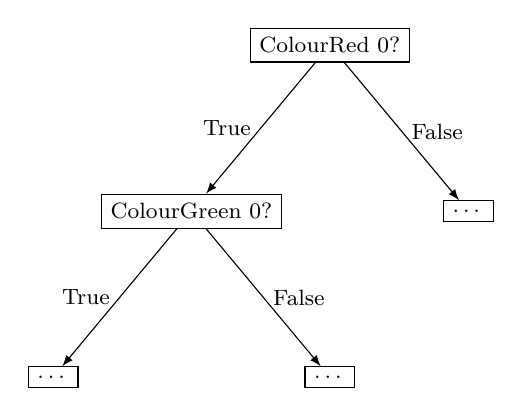
\begin{tikzpicture}
        [
            boxed/.style            = {shape=rectangle, draw, align=center},
            sibling distance        = 10em,
            level distance          = 6em,
            edge from parent/.style = {draw, -latex},
            every node/.style       = {font=\footnotesize},
        ]
        \node [boxed] {ColourRed $\leqslant 0$?}
            child { node [boxed] {ColourGreen $\leqslant 0$?}
                child { node [boxed] {\ldots} edge from parent node [left] {True} }
                child { node [boxed] {\ldots} edge from parent node [right] {False} }
                edge from parent node [left] {True} 
            }
            child { node [boxed] {\ldots} edge from parent node [right] {False} };
    \end{tikzpicture}
\end{center}
\caption{Reprise of the colour example where the data has been pre-processed using a one-hot encoding. Compared to \autoref{fig:categorical_binsplit} the structure is mirrored and the node names are less clear, but the essence remains the same.}%
\label{fig:colour_onehot}
\end{figure}

Alternatively, the label encoder would replace this categorical attribute with a single numerical attribute with possible values 0, 1 and 2. This implies that there is an order among the colours, which is not supposed to be the case. Tests such as $(x \leqslant 1.5)$ could be generated. This is equivalent to ``Colour is Red or Green?'', which is more expressive then what was possible so far. That looks positive at first, but not all logical combinations can be representation this way. In this example, no threshold can be found that implies ``Colour is Red or Blue''. Even worse, what can be represented depends entirely on the implied yet non-existent order of the original categorical variable. In short, this technique does not adhere to the original semantics and should not be used.

In conclusion, the suggested workaround with the one-hot encoder is acceptable but that does not change the fact that it negatively impact two of the decision tree advantages we listed earlier in \autoref{cha:intro}: no data preparation required and excellent comprehensibility.

\subsubsection{Missing values}
Another important input capability is dealing with missing values. As stated before, decision trees have fairly straightforward ways of dealing with this problem. While the papers on ID3 ignored this issue, both C4.5 and CART have methods for dealing with it. As before, Weka inherited the capability from C4.5, but scikit-learn did not inherit the same from CART. This is another case where extra pre-processing is needed to make decision tree induction work with scikit-learn. During this process, valuable observations might be thrown out entirely.

\subsection{Output capabilities}
\subsubsection{Classification and regression}
For this thesis regression is out of scope, but it is still an important point. CART has both classification and regression in its name, so it comes as no surprise that both are supported by this algorithm. The scikit-learn implementation is split in a \texttt{DecisionTreeClassifier} and a \texttt{DecisionTreeRegressor}. C4.5 only supports classification out of the box. Consequently, regression is not a capability of Weka's J48 implementation. However, Weka contains other decision tree algorithms, some of which do accommodate regression (e.g., \texttt{REPTree}).

\subsubsection{Multiclass, multilabel, multioutput}
On this front, scikit-learn is the superior implementation because all variants of multiclass, multilabel and multioutput are supported. Weka's J48 implementation on the other hand only supports multiclass. CART and C4.5 have the same limitations as Weka's. A simple workaround for multioutput is to fit multiple trees instead, although this might impact various performance aspects.

\subsection{Splitting criteria}
Another difference lies in the choice of splitting criteria. C4.5 and J48 support the typical criteria based on information theory such as information gain and gain ratio. CART and scikit-learn on the other hand both support information gain and the Gini impurity index but not gain ratio since it is not beneficial for binary trees. The purity criterion is not implemented in any of the algorithms due to its poor performance.

\subsection{Early stopping and pruning}
As mentioned at the end of \autoref{cha:literature}, both C4.5 and CART seemingly have their favourite pruning algorithms. The former explicitly supports Error Based Pruning and Rule-based Pruning, while the latter favours Cost Complexity Pruning. J48, like C4.5, supports Error Based Pruning by default. Quinlan's other proposal, Reduced Error Pruning, is also an option. Rule-based pruning is not supported, but Weka contains other rule based algorithms as an alternative. Of course the option not to prune at all is also available. In that case users can fall back on early stopping criteria. All algorithms and implementations include some simple stopping criteria. ID3 also introduced more complex stopping criteria, but that effort was abandoned in favour of pruning in C4.5. Breiman came to the same conclusion for CART. Surprisingly, scikit-learn did not follow Breiman's suggestion of implementing Cost Complexity Pruning. Instead, it opted for the inferior practice of using simplistic early stopping criteria such as a maximum tree depth or a minimum number of observations per node required to split it. This is by far the most significant difference between the two implementations.

\subsection{Mode of operation}
Machine learning algorithms typically operate in either one of two modes: online or offline (batch) mode. None of the algorithms and implementations under scrutiny offer online learning. Weka does include an implementation of an online tree builder (i.e., a HoeffdingTree), but not as part of J48.

\subsection{Miscellaneous}
Many more capabilities exist, but these are beyond the scope of this thesis. The interested reader can dive deeper into any of the following topics:
\begin{itemize}
    \item Generating rulesets starting for a tree representation
    \item Assigning different weights to different classes
    \item Assigning different weights to different observations
    \item Taking asymmetric misclassification costs into account
\end{itemize}

\subsection{Summary}

\begin{figure}[p]
    \centering
    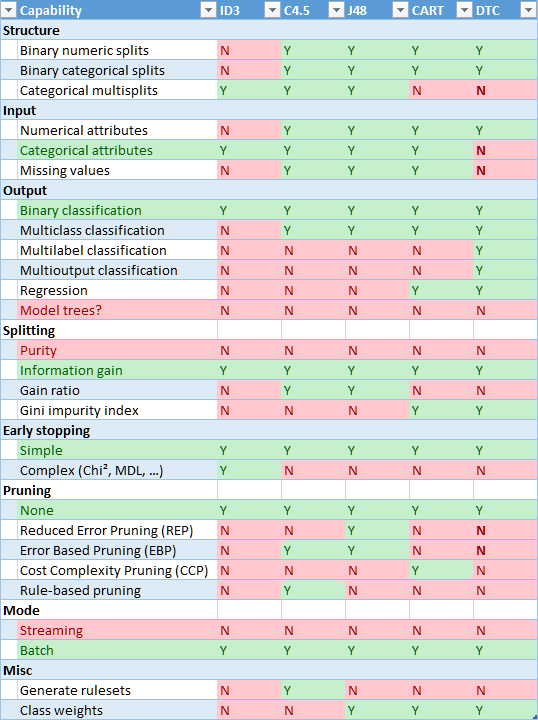
\includegraphics[width=\textwidth]{img/capabilities.png}
    \caption{Summary of various capabilities as seen in the ID3, C4.5 and CART algorithms, but also in their implementations: Weka's J48 and scikit-learn's \texttt{DecisionTreeClassifier} (DTC).}%
    \label{fig:capabilities}
\end{figure}
%TODO replace with prettier visualization

Figure~\ref{fig:capabilities} shows a summary of the previous paragraphs. During the comparison of capabilities of the C4.5 and CART algorithms and their respective software counterparts Weka J48 and scikit-learn's \texttt{DecisionTreeClassifier}, three important discrepancies at the expense of the latter came up. 
\begin{itemize}
    \item It lacks pruning algorithms, making it rely on inferior simple stopping criteria instead.
    \item It cannot handle categorical attributes natively. This specifically impacts its capability of making categorical multisplits.
    \item It fails when given a training set with missing data.
\end{itemize}

Other discrepancies came up, but these were either minor or could be rationalized as explained in the previous paragraphs.

\section{Next steps}

\subsection{Lack of pruning}
The lack of pruning is a particularly noteworthy discrepancy. The current workaround involves carefully defining early stopping criteria. However, it is clearly established in the literature that this workaround is inferior to the usage of proper pruning algorithms~\cite{cart, c45}. Fixing this is priority number one. Fixing in this sense means implementing pruning algorithms for the scikit-learn decision tree induction algorithms. The next chapter immediately discusses this in more detail. In later chapters, we propose an experimental setup to evaluate the performance of the new implementation and present the results of that evaluation. Our hypothesis: pruned trees take longer to train but are smaller. That makes them less prone to overfitting so the accuracy should be the same or better and the prediction time should decrease.

\subsection{Categorical attribute handling}\label{ssec:cat_attr_handling}
Next to the lack of pruning, scikit-learn's algorithms also have a problem with categorical input. Because scikit-learn is built on top of NumPy, it uses numerical matrices to pass data between all its components. As such, categorical data simply cannot serve as input to most of its algorithms. It is part of the core philosophy of scikit-learn. Fixing this head-on would require a complete rewrite of not only the decision tree algorithms, but also all the basic interfaces and their dependencies, which is far beyond the scope of this thesis. On top of that, the use of NumPy is essential for the performance of scikit-learn. Python in itself is a slow, interpreted scripting language that is not suited for high performance computing tasks. Its integration options with C code (and the intermediate Cython code) make it a viable option, but at a considerable development cost. NumPy abstracts this complexity away behind a pure, easy to use Python interface while maintaining the speed boost.

A less significant but related discrepancy is that scikit-learn's decision tree induction implementation only generates binary trees. Breiman made this conscious choice for his CART algorithm in 1984, and it remains so today in its derivatives. Fixing this once again fundamentally changes the implementation and therefore entails a complete rewrite of the decision tree package.

In conclusion, the currently accepted workaround of pre-processing the categorical attributes in the input data using a one-hot encoder seems to be our best bet. In the upcoming chapters, we design an experiment that tests whether this workaround has any performance implications. Given the isomorphism between binary tests based on categorical attributes and binary tests based on numerical values that are the result of a one-hot encoding, we hypothesize that the performance impact is limited.

\subsection{Missing value handling}
The third and lowest priority problem is the failure of scikit-learn to process datasets containing missing values. Three approaches are possible. The first workaround discards any observation with missing values. Depending on the context, this data loss is somewhere between irrelevant and unacceptable. The second workaround attempts to guess the values for the gaps in the data based on the rest of the data. The user must judge whether this approach is feasible in his context, but it certainly is no universal solution. For that, we look at the third option. Unlike the previous workarounds, this is not a pre-processing step. Instead, the classifier itself must be modified to deal with missing data directly. Decision tree induction algorithms typically have that capability. The C4.5 and CART texts both outline ways to deal with this problem. One option is to split an observation with a missing value into as many pseudo observations as there are possible values for the missing (categorical) attribute where each distinct value is used once. Some lower internal weight could be assigned to these pseudo observations to compensate for the data expansion.

\section{Conclusion}
This chapter introduced us to the various capabilities of decision trees. Those capabilities were mapped onto both the CART and C4.5 algorithms, but also the Weka J48 and scikit-learn implementations. This exercise revealed three important discrepancies that make scikit-learn inferior to Weka regarding decision tree induction. Those discrepancies concern pruning, categorical values and missing values. For each of these, next steps have been defined. The next chapter immediately tackles the pruning problem head-on.
